\section{Test: Linear model}
The purpose of this chapter is to show and discuss the performance results of the LQI controller derived in \cref{sec:ctrl-design} on the linear model derived in \cref{sec:linear_model}. The controller is benchmarked against the original FLC controller with regards to both rotor speed control and fore-aft movement dampening capability. Prior to the test the LQI controller has been tuned such that a satisfactory performance was achieved on the linear model. 

It is naturally expected that the LQI controller will perform much better in damping the fore-aft movement than the original FLC. It is also expected to perform better in generator speed control despite the fact that the original FLC controller has been thoroughly tuned to achieve the best possible generator speed tracking performance. The reason for this is that the LQI controller has been tuned on the simple linear model and not in VTS. Thus potential unforeseen consequences of having an aggressive controller in a more realistic environment are not discovered until it is tested in VTS.

Test results are shown for both frequency and time domain.

\subsection{Test framework}



\subsection{Test results}

\subsubsection{Frequency Domain}
The fre

\begin{figure}[ht]
	\centering
	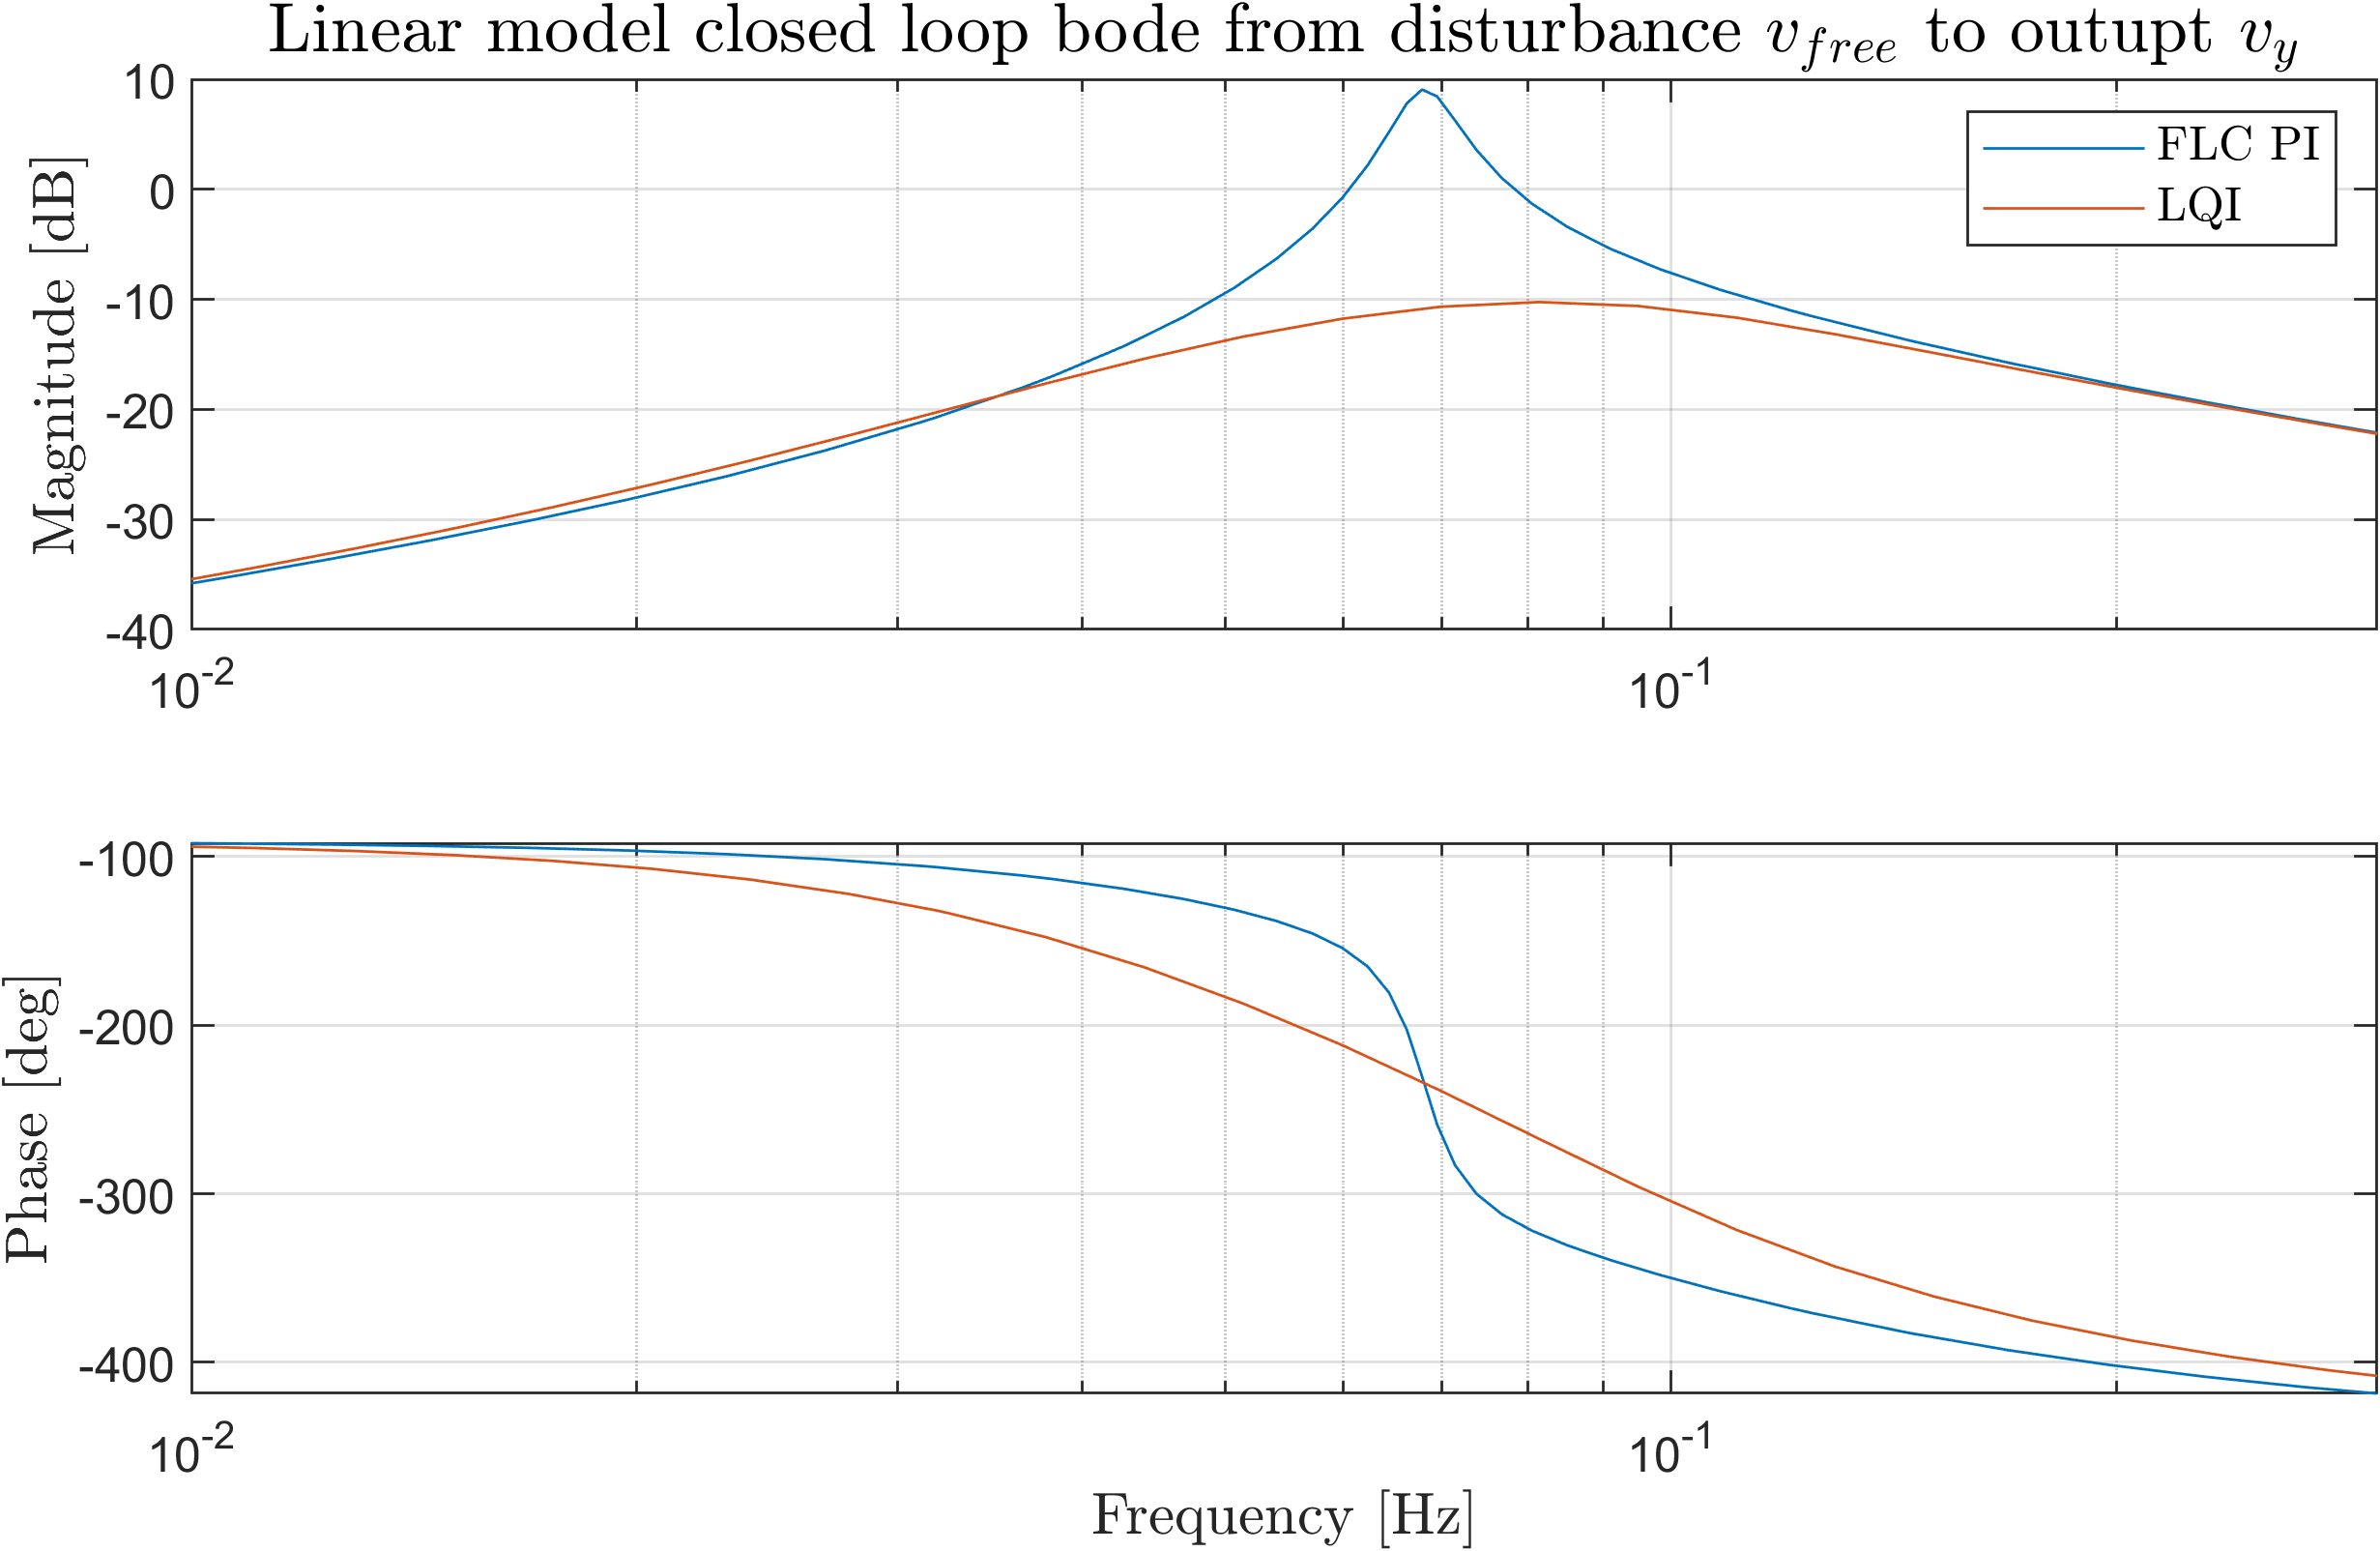
\includegraphics[width=0.7\linewidth]{Graphics/TestResults/linearModPerf/10_vfreeTovy.png}
	\caption{Frequency response from the free wind as observed by the rotor ($ v_{free} $) to the rotor speed  ($ \Omega $) of the linear model with comparison between the original FLC PI controller and the developed LQI controller.}
	\label{fig:10_vfreeTovy}
\end{figure}

\begin{figure}[ht]
	\centering
	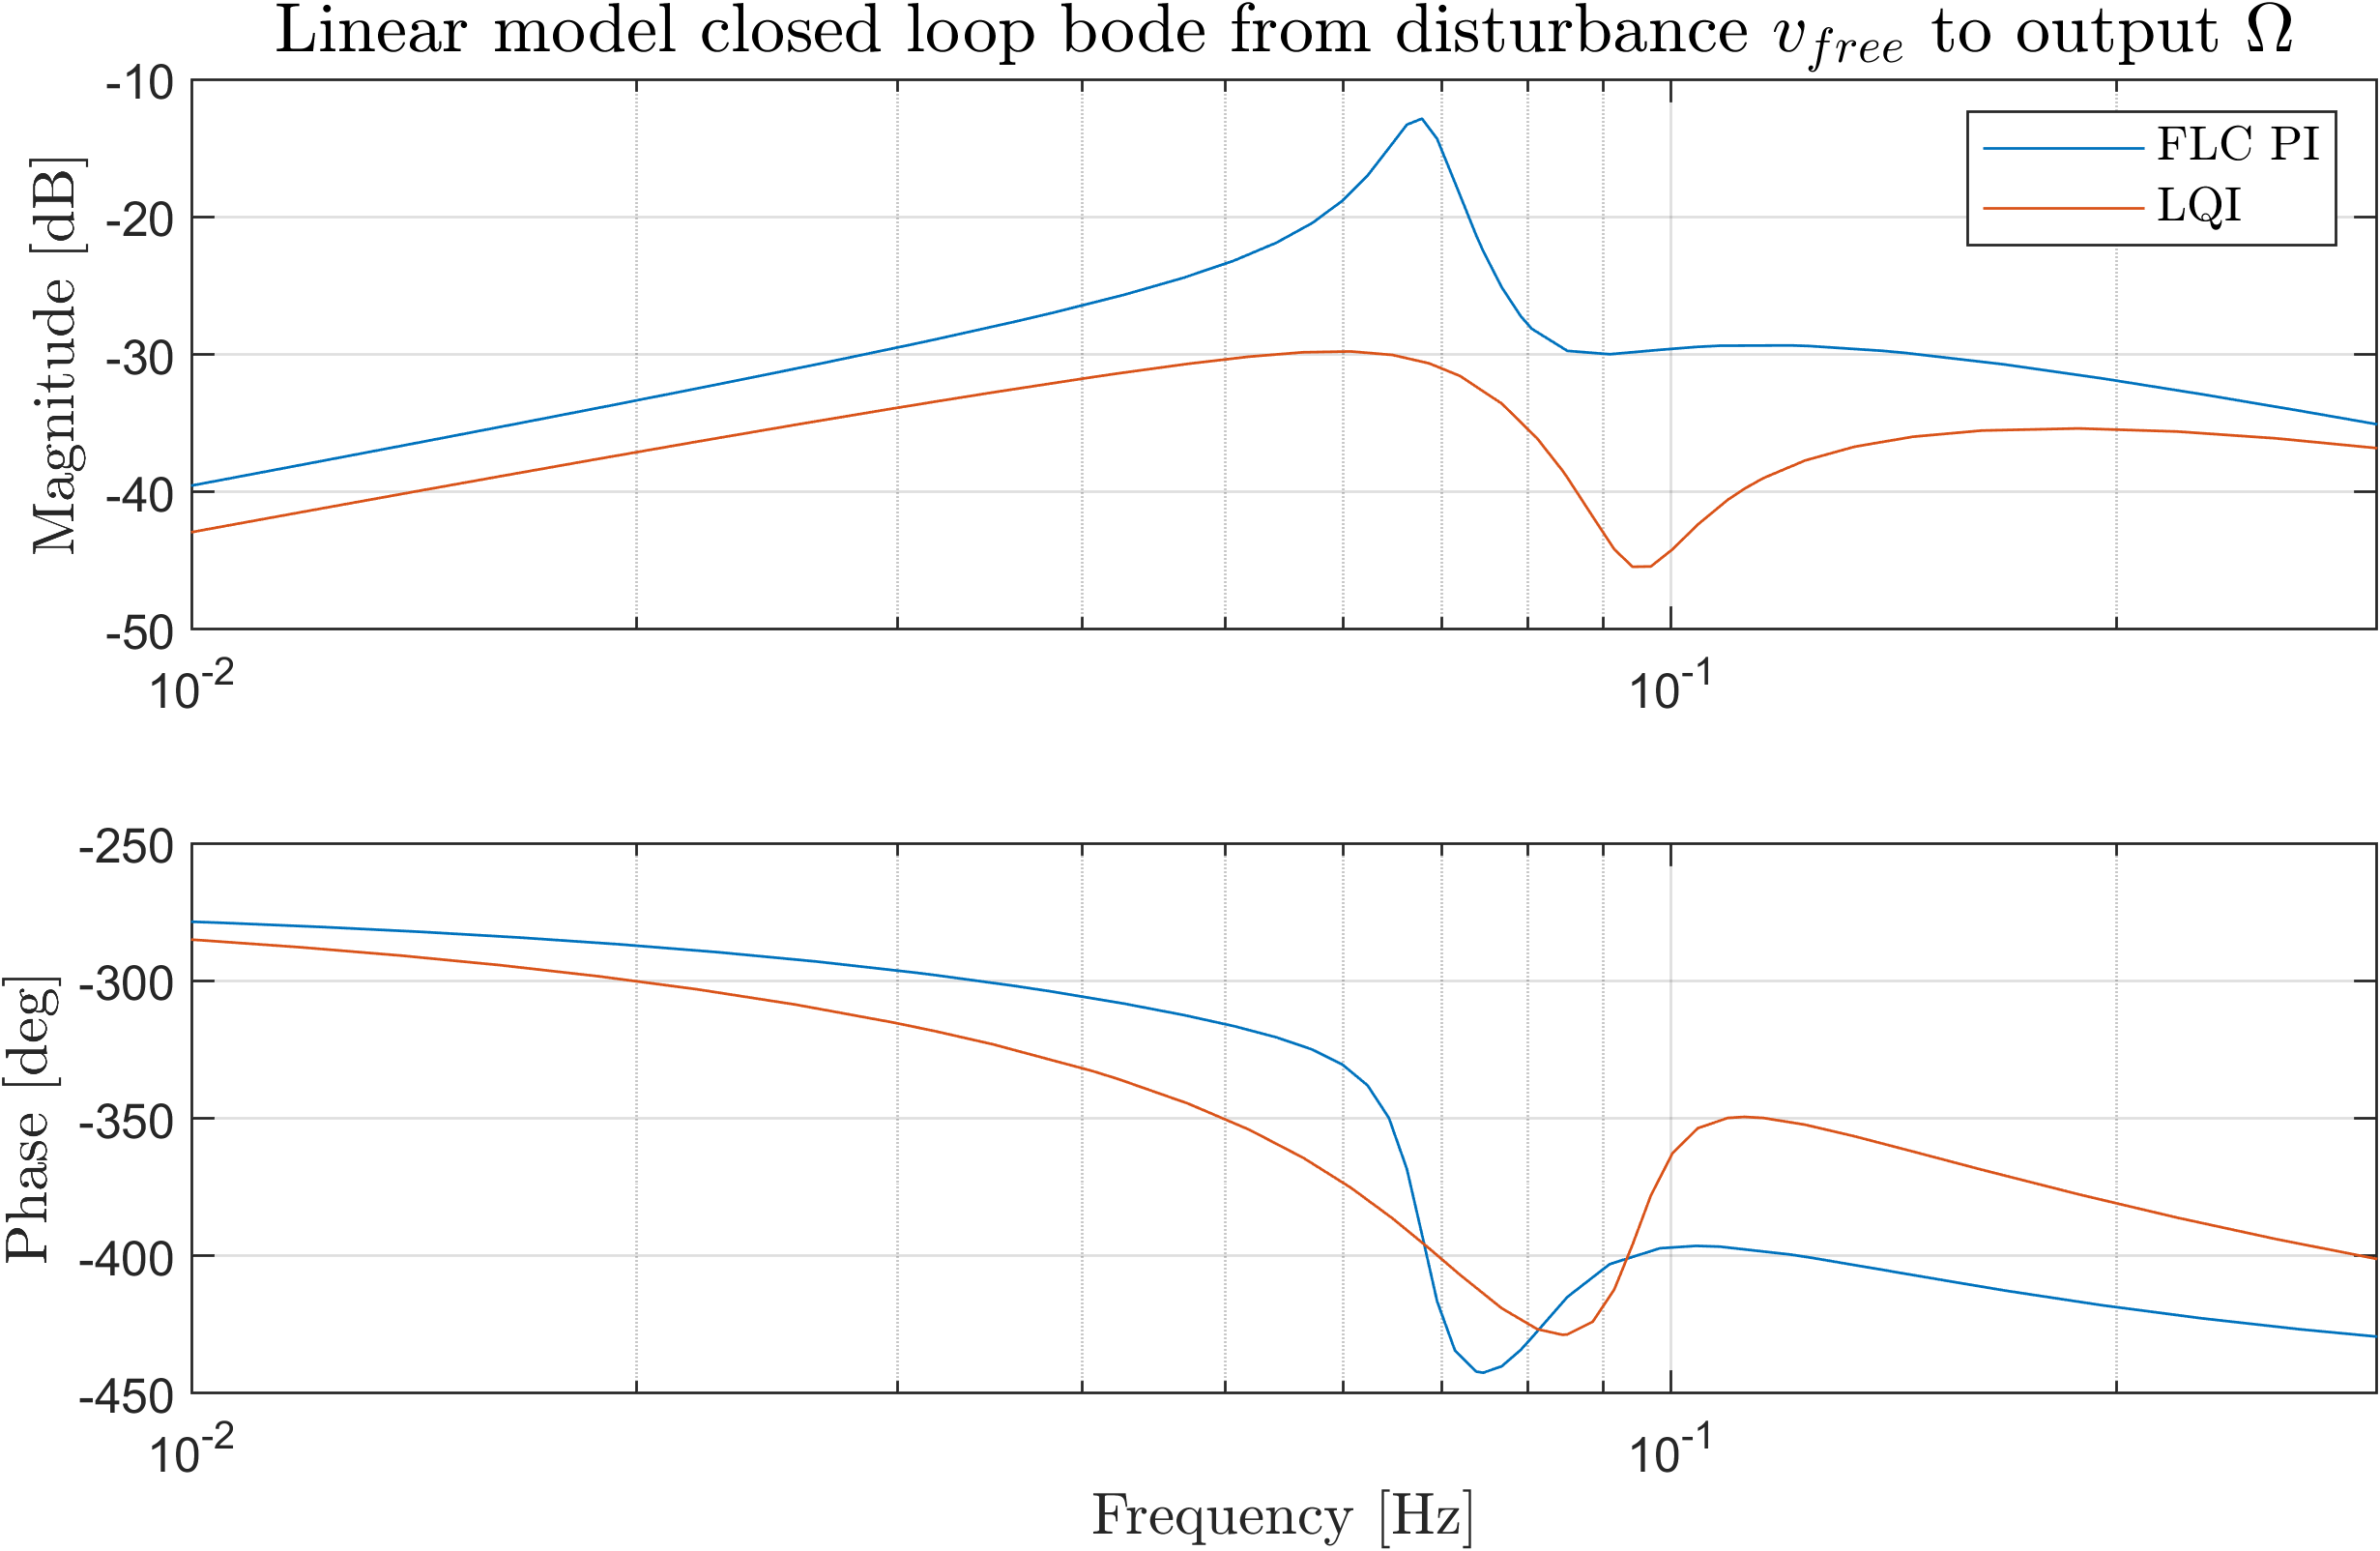
\includegraphics[width=0.7\linewidth]{Graphics/TestResults/linearModPerf/11_vfreeToW.png}
	\caption{Frequency response from the free wind as observed by the rotor ($ v_{free} $) to the surge direction tower top velocity ($ v_y $) of the linear model with comparison between the original FLC PI controller and the developed LQI controller.}
	\label{fig:11_vfreeToW}
\end{figure}


\subsubsection{Time domain}

\begin{figure}[ht]
	\centering
	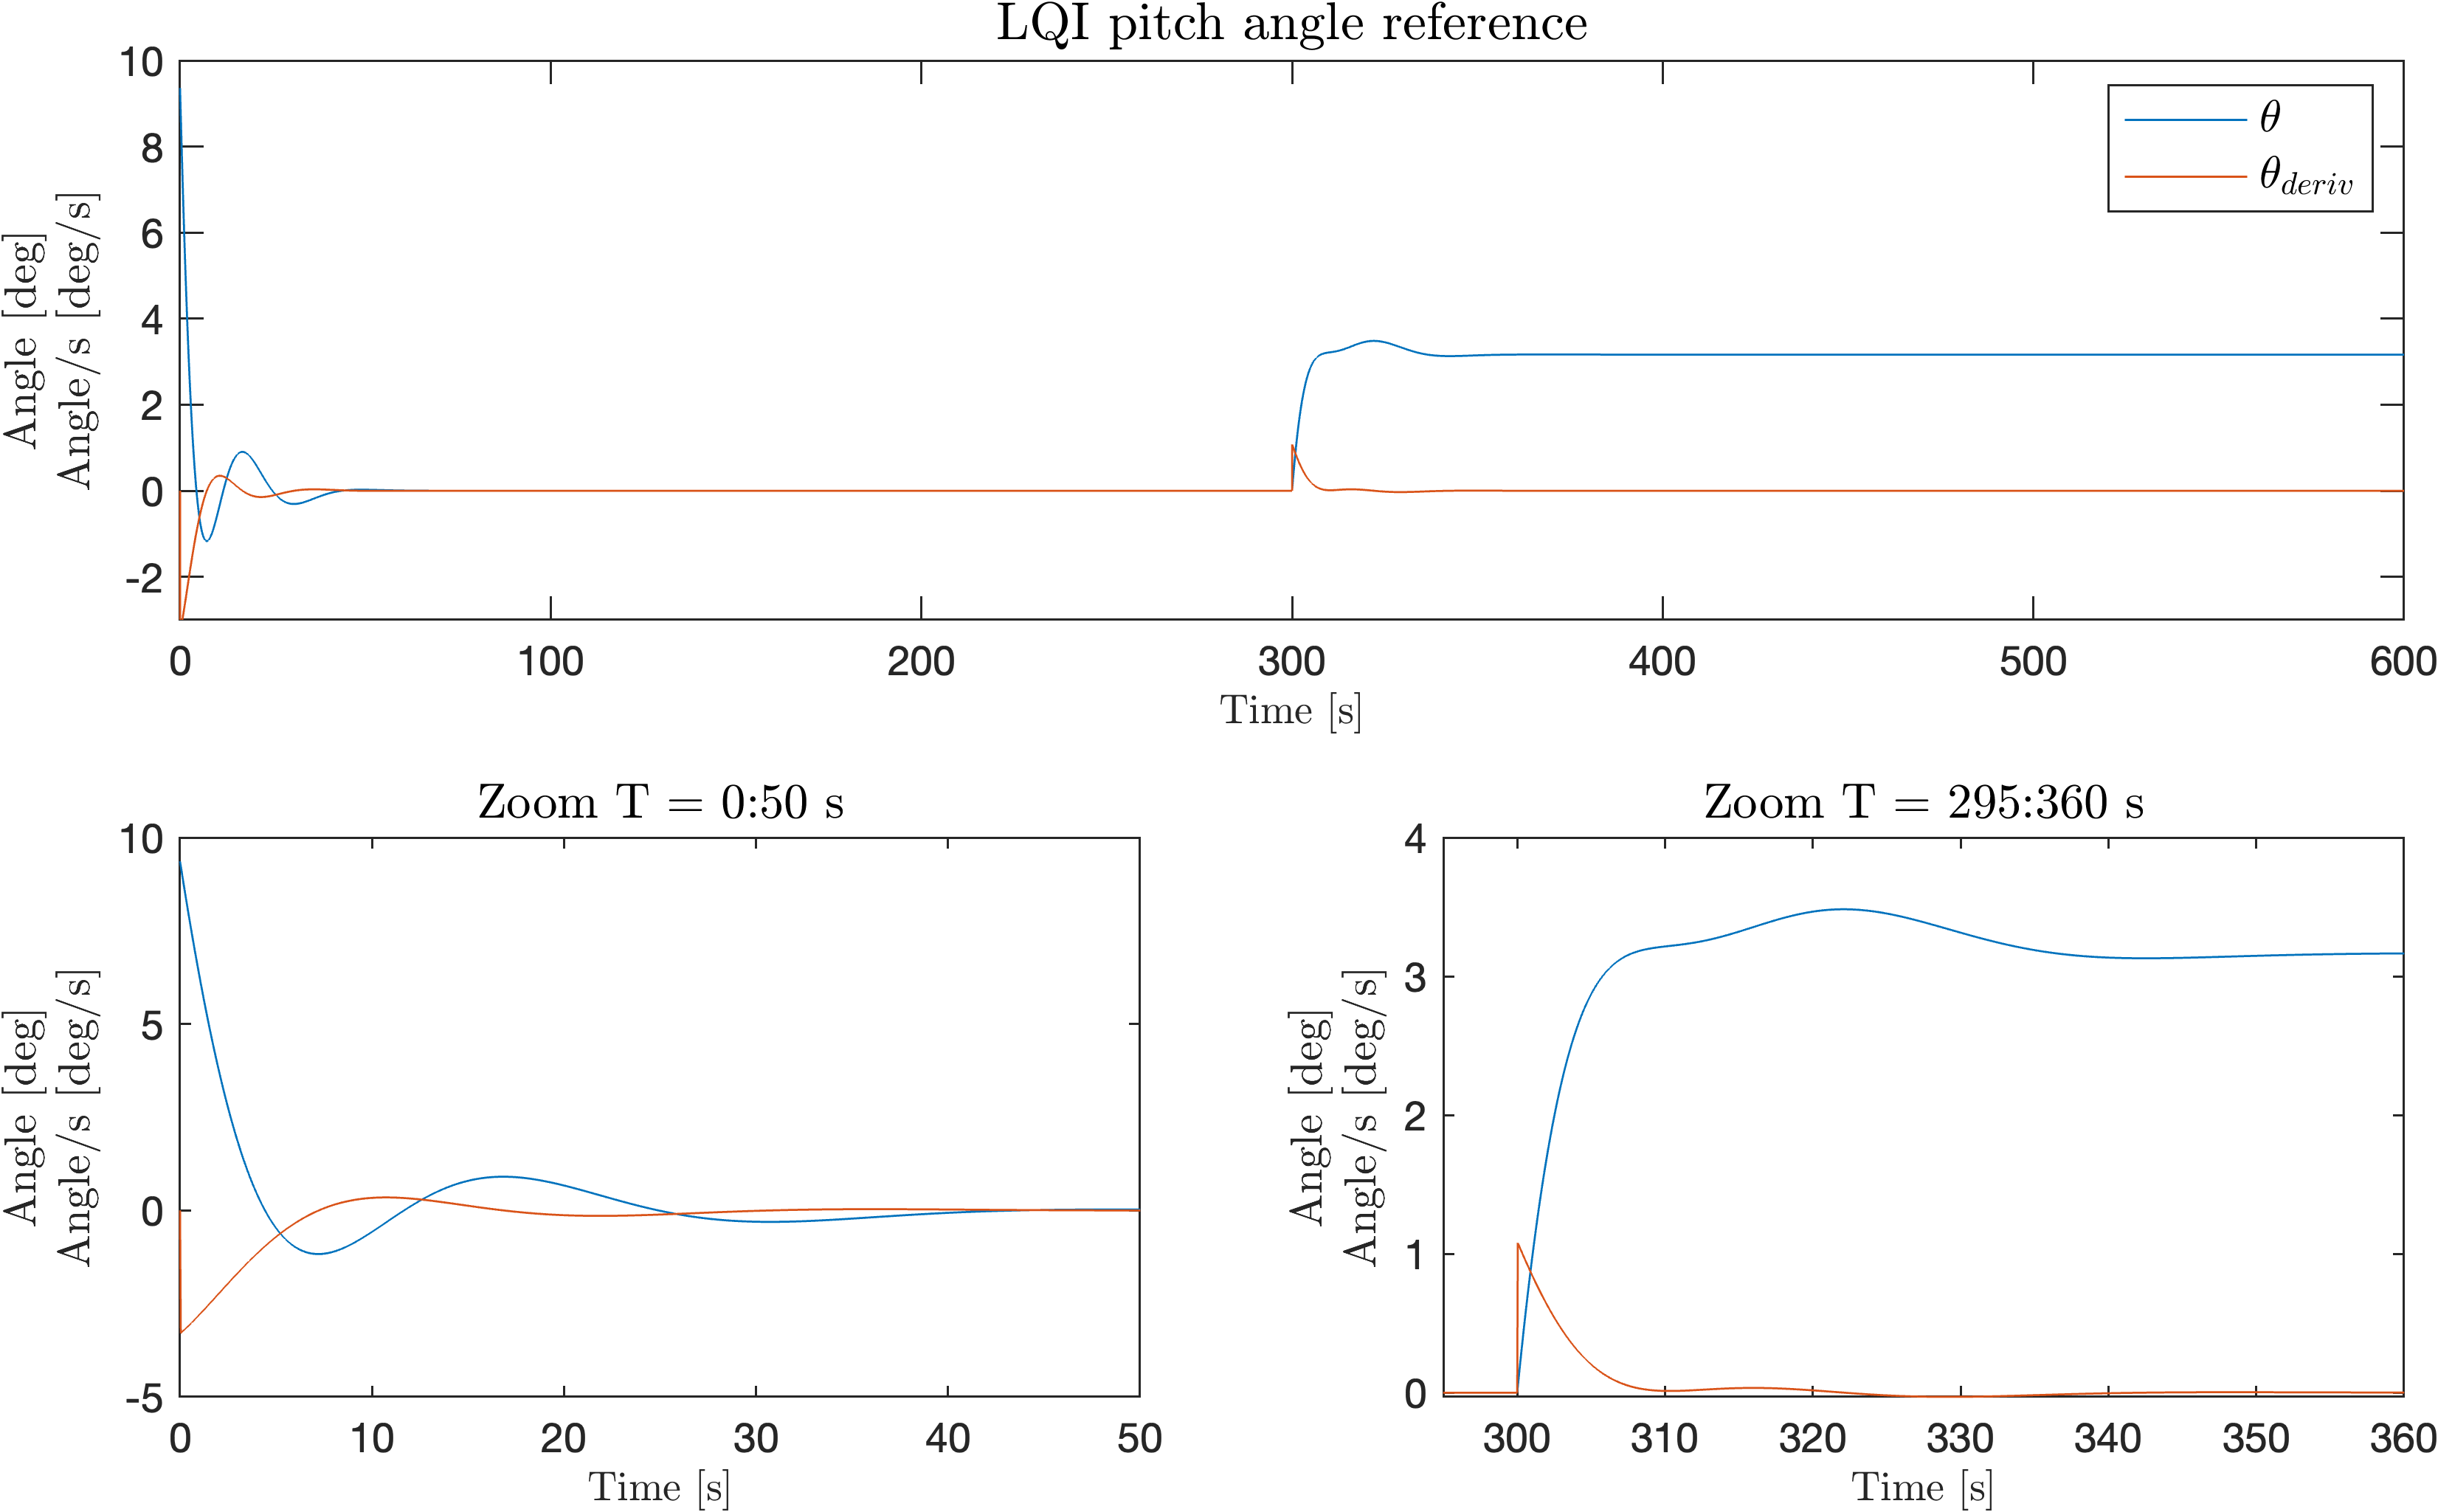
\includegraphics[width=0.7\linewidth]{Graphics/TestResults/linearModPerf/01_pitch.png}
	\caption{}
	\label{fig:01_pitch}
\end{figure}

\begin{figure}[ht]
	\centering
	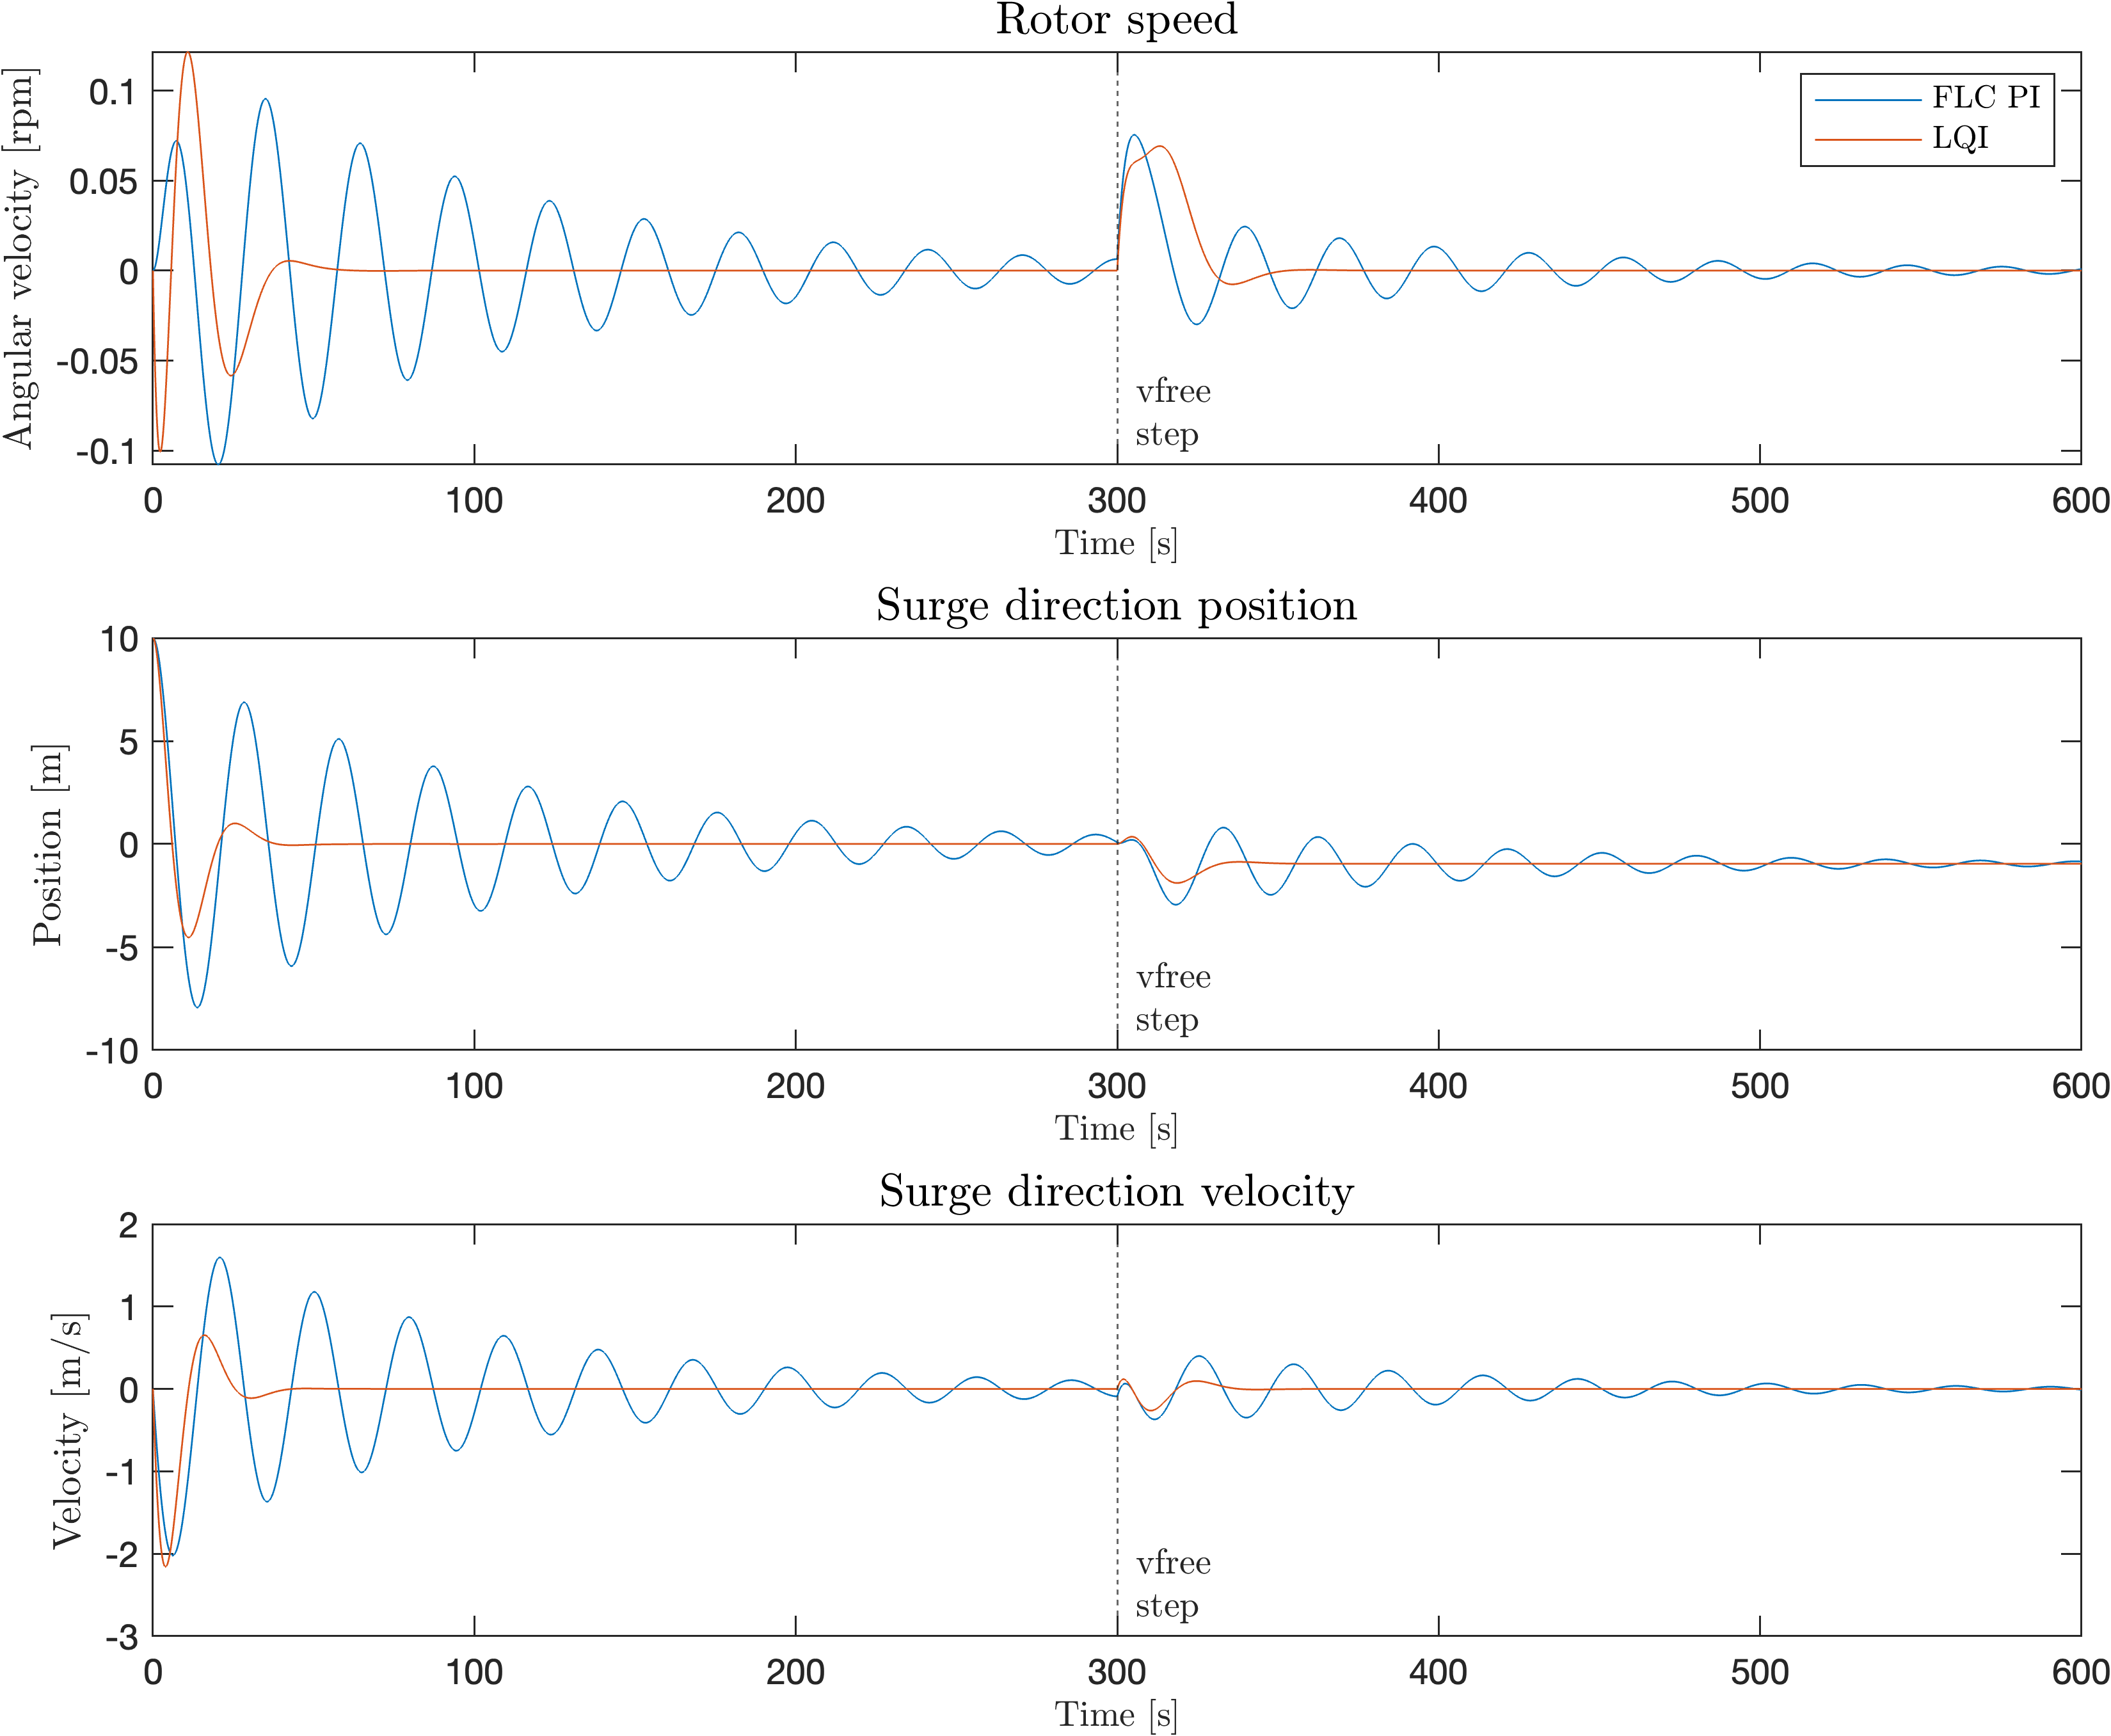
\includegraphics[width=0.7\linewidth]{Graphics/TestResults/linearModPerf/02_W_py_vy_comp.png}
	\caption{}
	\label{fig:02_W_py_vy_comp}
\end{figure}

\begin{figure}[ht]
	\centering
	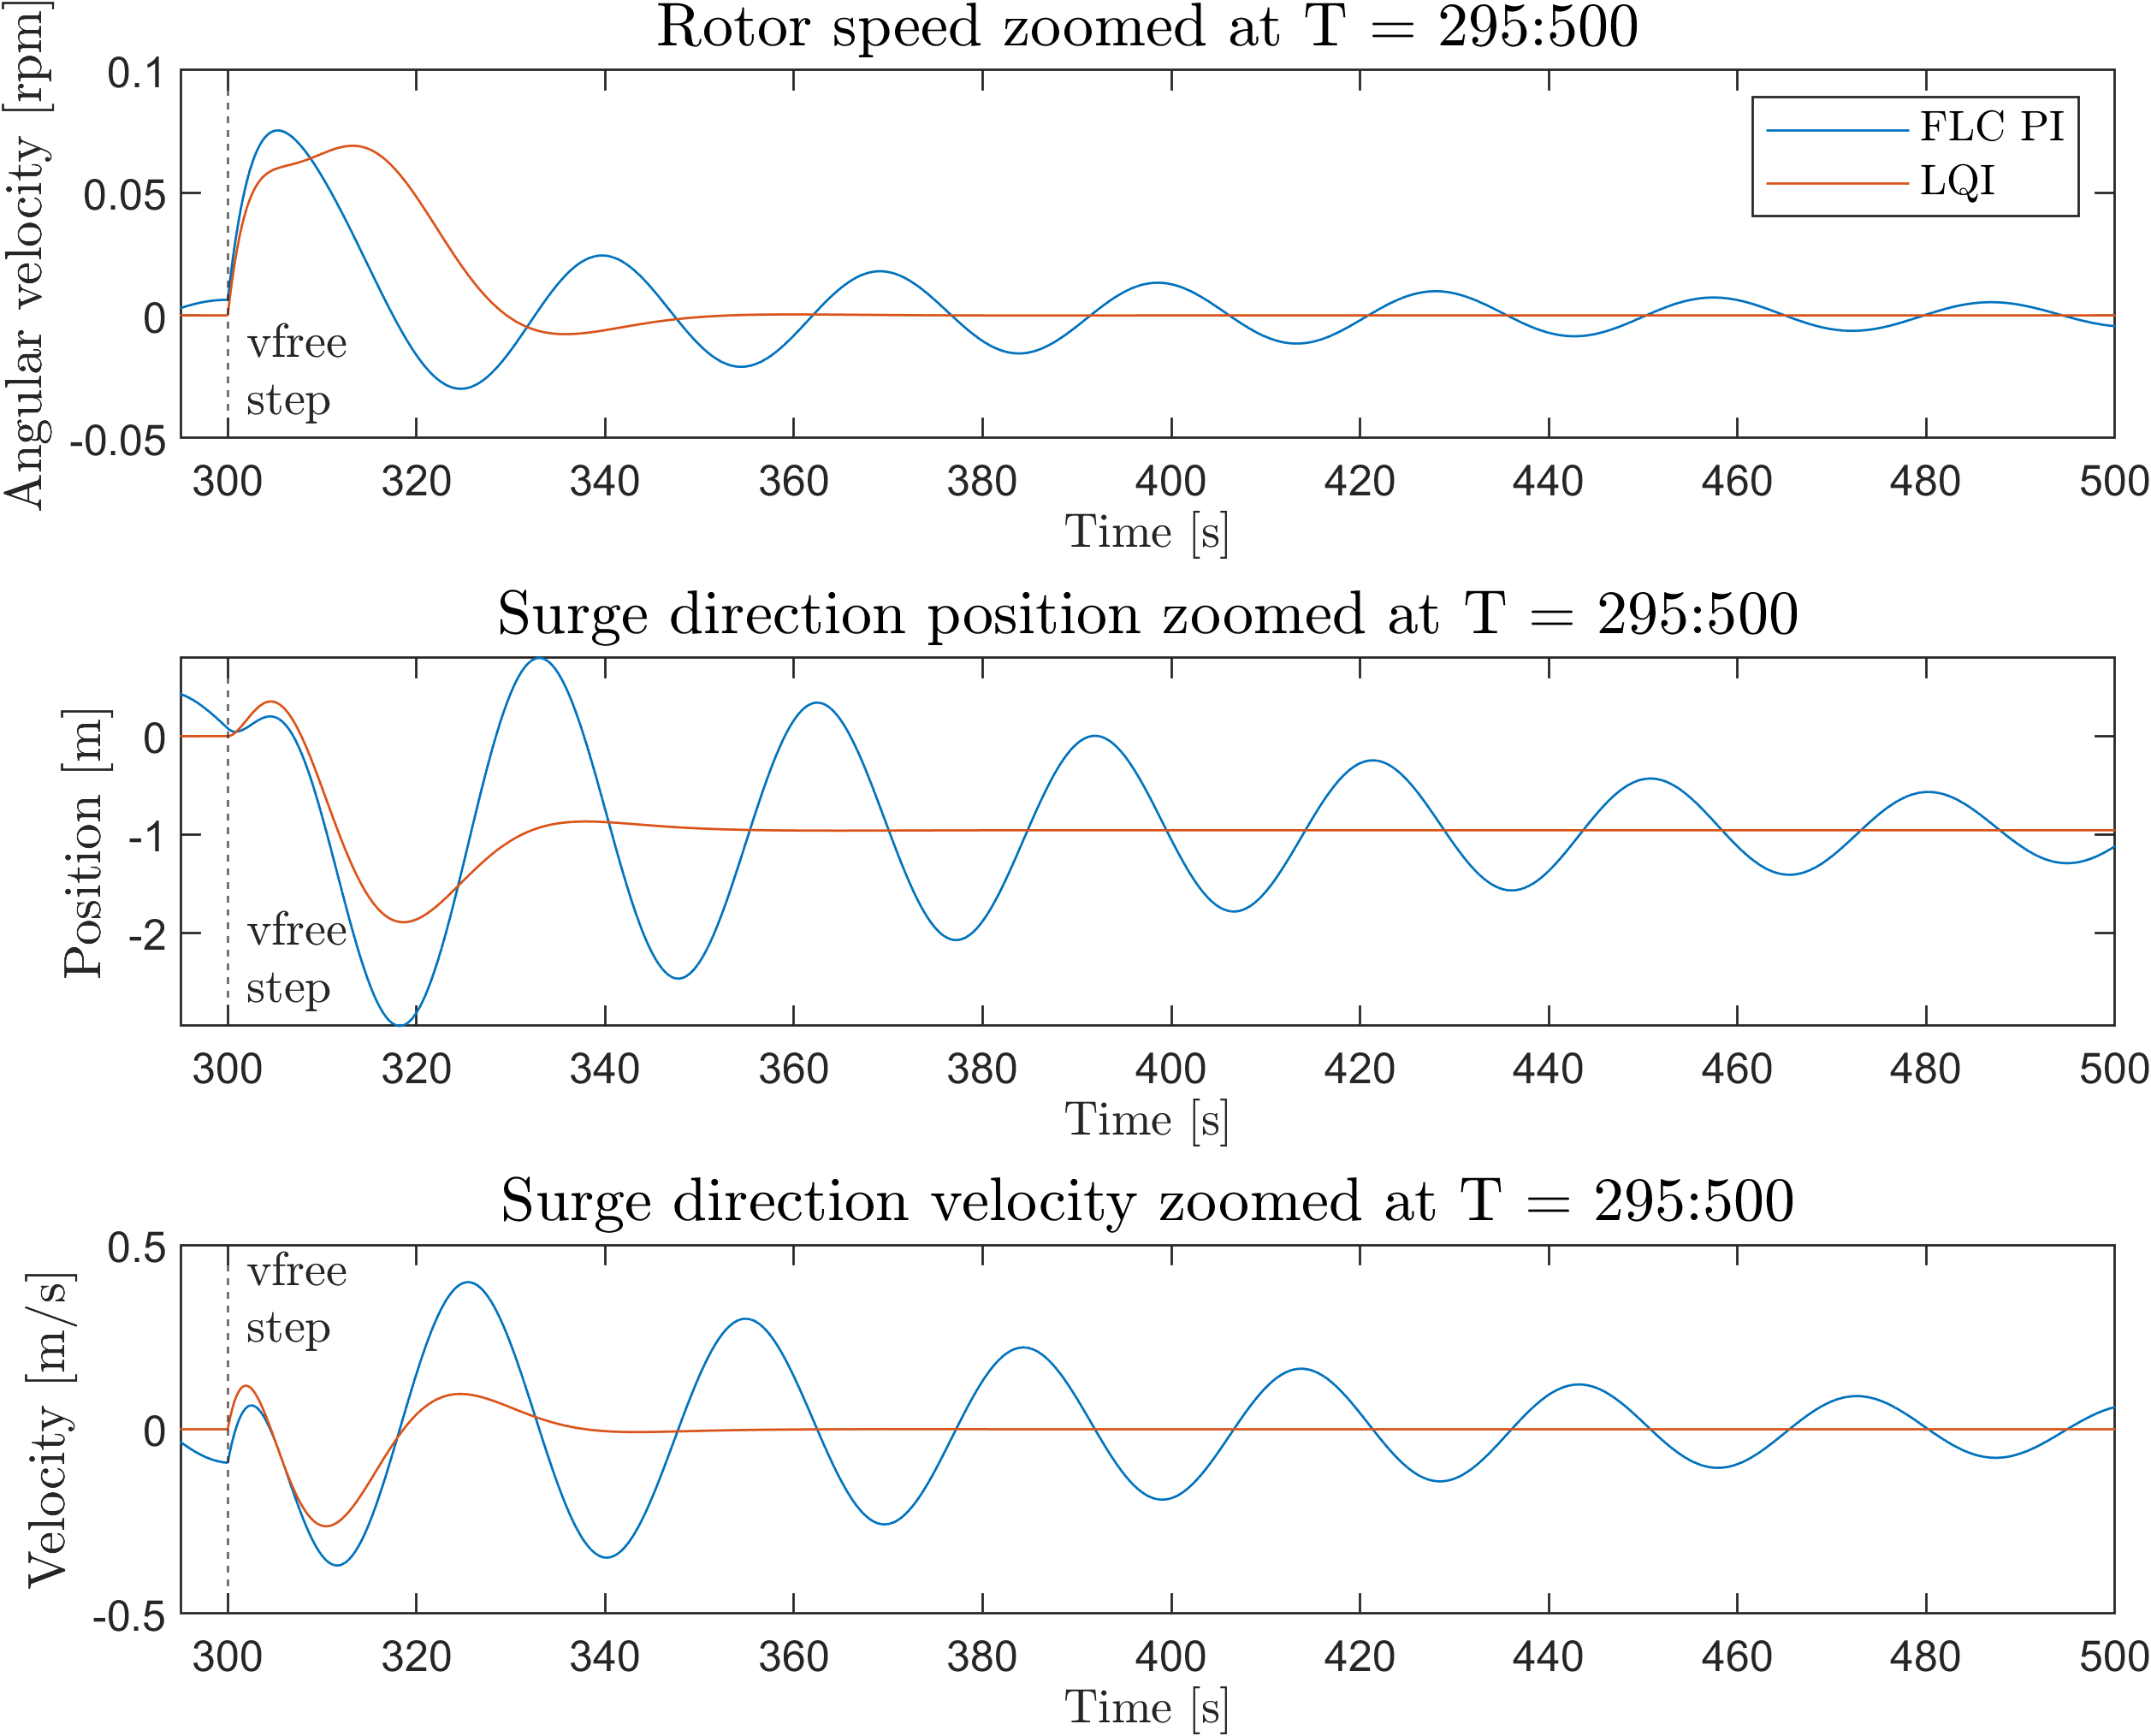
\includegraphics[width=0.7\linewidth]{Graphics/TestResults/linearModPerf/03_W_py_vy_comp_zoom.png}
	\caption{}
	\label{fig:03_W_py_vy_comp_zoom}
\end{figure}